
%{{第二十六回}}{第二十六回}}

\chapter{蜂腰桥设言传蜜意 潇湘馆春困发幽情}\label{part0030_split_000.htmlux5cux23calibre_pb_0}

{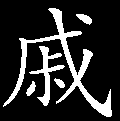
\includegraphics[width=3mm]{../Images/00005}一个是时才得传消息,一个是旧喜化作新歌。真真假假事堪疑,哭向花林月底。}

话说宝玉养过了三十三天之后,不但身体强壮,亦且连脸上疮痕平复,仍回大观园内去。这也不在话下。

且说近日宝玉病的时节,贾芸带着家下小厮坐更看守,昼夜在这里,那红玉同众丫鬟也在这里守着宝玉,彼此相见多日,都渐渐的混熟了。那红玉见贾芸手里拿的手帕子,倒像是自己从前掉的,待要问他,又不好问的。不料那和尚、道士来过,用不着一切男人,贾芸仍种树去了。这件事待要放下,心内又放不下,待要问去,又怕人猜疑,正是犹豫不决、神魂不定之际,忽听窗外问道:``姐姐在屋里没有?''{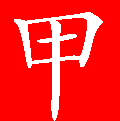
\includegraphics[width=3mm]{../Images/00002}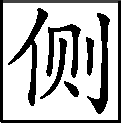
\includegraphics[width=3mm]{../Images/00011}\footnotesize \kaishu 岔开正文,却是为正文作引。 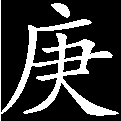
\includegraphics[width=3mm]{../Images/00004}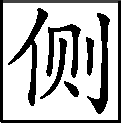
\includegraphics[width=3mm]{../Images/00011}\footnotesize \kaishu 你看他偏不写正文,偏有许多闲文,却是补遗。}红玉闻听,在窗眼内望外一看,原来是本院的小丫头名叫佳蕙的,因答说:``在家里,你进来罢。''佳蕙听了跑进来,就坐在床上,笑道:``我好造化!才刚在院子里洗东西,宝玉叫往林姑娘那里送茶叶,{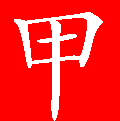
\includegraphics[width=3mm]{../Images/00002}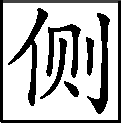
\includegraphics[width=3mm]{../Images/00011}\footnotesize \kaishu 交代井井有法。 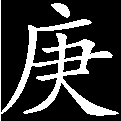
\includegraphics[width=3mm]{../Images/00004}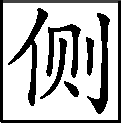
\includegraphics[width=3mm]{../Images/00011}\footnotesize \kaishu 前文有言。}花大姐姐交给我送去。可巧老太太那里给林姑娘送钱来,{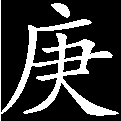
\includegraphics[width=3mm]{../Images/00004}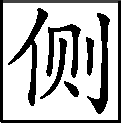
\includegraphics[width=3mm]{../Images/00011}\footnotesize \kaishu 是补写否?}正分给他们的丫头们呢。{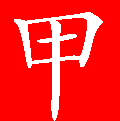
\includegraphics[width=3mm]{../Images/00002}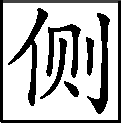
\includegraphics[width=3mm]{../Images/00011}\footnotesize \kaishu 潇湘常事出自别院婢口中,反觉新鲜。}见我去了,林姑娘就抓了两把给我,也不知多少。你替我收着。''便把手帕子打开,把钱倒了出来,红玉替他一五一十的数了收起。{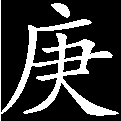
\includegraphics[width=3mm]{../Images/00004}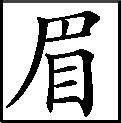
\includegraphics[width=3mm]{../Images/00010}\footnotesize \kaishu 此等细事是旧族大家闺中常情,今特为暴发钱奴写来作鉴。一笑。壬午夏,雨窗。}

佳蕙道:``你这一程子心里到底觉怎么样?依我说,你竟家去住两日,请一个大夫来瞧瞧,吃两剂药就好了。''红玉道:``那里的话,好好的,家去作什么!''佳蕙道:``我想起来了,林姑娘生的弱,时常他吃药,{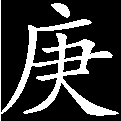
\includegraphics[width=3mm]{../Images/00004}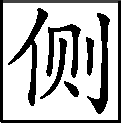
\includegraphics[width=3mm]{../Images/00011}\footnotesize \kaishu 是补写否?}你就和他要些来吃,也是一样。''{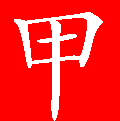
\includegraphics[width=3mm]{../Images/00002}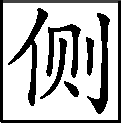
\includegraphics[width=3mm]{../Images/00011}\footnotesize \kaishu 闲言中叙出黛玉之弱。草蛇灰线。}红玉道:``胡说!药也是混吃的。''{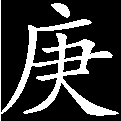
\includegraphics[width=3mm]{../Images/00004}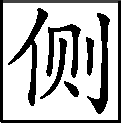
\includegraphics[width=3mm]{../Images/00011}\footnotesize \kaishu 如闻。}佳蕙道:``你这也不是个长法儿,又懒吃懒喝的,终久怎么样?''{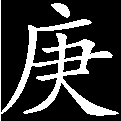
\includegraphics[width=3mm]{../Images/00004}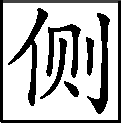
\includegraphics[width=3mm]{../Images/00011}\footnotesize \kaishu 从旁人眼中口中出,妙极!}红玉道:``怕什么,还不如早些儿死了倒干净!''{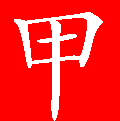
\includegraphics[width=3mm]{../Images/00002}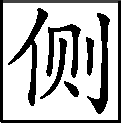
\includegraphics[width=3mm]{../Images/00011}\footnotesize \kaishu 此句令人气噎,总在无可奈何上来。}佳蕙道:``好好的,怎么说这些话?''红玉道:``你那里知道我心里的事!''

佳蕙点头想了一会,道:``可也怨不得,这个地方难站。就像昨儿老太太因宝玉病了这些日子,{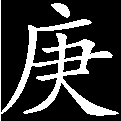
\includegraphics[width=3mm]{../Images/00004}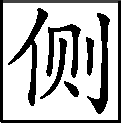
\includegraphics[width=3mm]{../Images/00011}\footnotesize \kaishu 是补文否?}说跟着伏侍的这些人都辛苦了,如今身上好了,各处还完了愿,{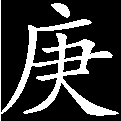
\includegraphics[width=3mm]{../Images/00004}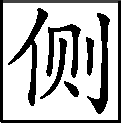
\includegraphics[width=3mm]{../Images/00011}\footnotesize \kaishu 是补写否?}叫把跟着的人都按着等儿赏他们。{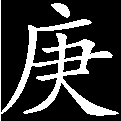
\includegraphics[width=3mm]{../Images/00004}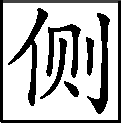
\includegraphics[width=3mm]{../Images/00011}\footnotesize \kaishu 是补写否?}我算年纪小,上不去,不得我也不怨;像你怎么也不算在里头?{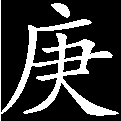
\includegraphics[width=3mm]{../Images/00004}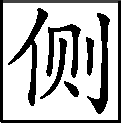
\includegraphics[width=3mm]{../Images/00011}\footnotesize \kaishu 道着心病。}我心里就不服。袭人那怕他得十个分儿,也不恼他,原该的。说良心话,谁还敢比他呢?{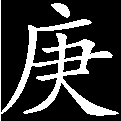
\includegraphics[width=3mm]{../Images/00004}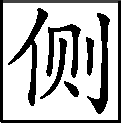
\includegraphics[width=3mm]{../Images/00011}\footnotesize \kaishu 确论公论,方见袭卿身份。}别说他素日殷勤小心,便是不殷勤小心,也拼不得。可气晴雯、绮霰他们这几个,都算在上等里去,仗着老子娘的脸面,众人倒捧着他去。你说可气不可气?''红玉道:``也不犯着气他们。俗语说的,`千里搭长棚,没有个不散的筵席',{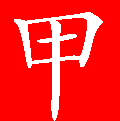
\includegraphics[width=3mm]{../Images/00002}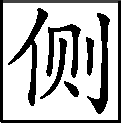
\includegraphics[width=3mm]{../Images/00011}\footnotesize \kaishu 此时写出此等言语,令人堕泪。}谁守谁一辈子呢?不过三年五载,各人干各人的去了。那时谁还管谁呢?''这两句话不觉感动了佳蕙的心肠,{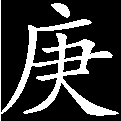
\includegraphics[width=3mm]{../Images/00004}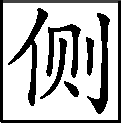
\includegraphics[width=3mm]{../Images/00011}\footnotesize \kaishu 不但佳蕙,批书者亦泪下矣。}由不得眼睛红了,又不好意思好端端的哭,只得勉强笑道:``你这话说的却是。昨儿宝玉还说,{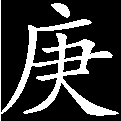
\includegraphics[width=3mm]{../Images/00004}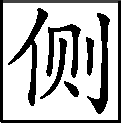
\includegraphics[width=3mm]{../Images/00011}\footnotesize \kaishu 还是补文。}明儿怎么样收拾房子,怎么样做衣裳,倒像有几百年的熬煎。''{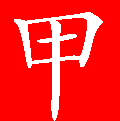
\includegraphics[width=3mm]{../Images/00002}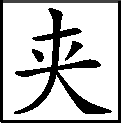
\includegraphics[width=3mm]{../Images/00012}\footnotesize \kaishu 却是小女儿口中无味之谈,实是写宝玉不如一鬟婢。}

红玉听了冷笑了两声,方要说话,{{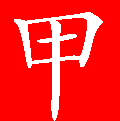
\includegraphics[width=3mm]{../Images/00002}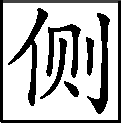
\includegraphics[width=3mm]{../Images/00011}\footnotesize \kaishu 文字又一顿。 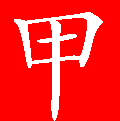
\includegraphics[width=3mm]{../Images/00002}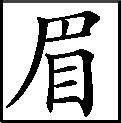
\includegraphics[width=3mm]{../Images/00010}\footnotesize \kaishu 红玉一腔委屈怨愤,系身在怡红不能遂志,看官勿错认为芸儿害相思也。}{[}己卯冬。{]}{ 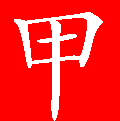
\includegraphics[width=3mm]{../Images/00002}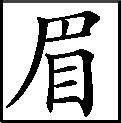
\includegraphics[width=3mm]{../Images/00010}\footnotesize \kaishu ``狱神庙''红玉、茜雪一大回文字惜迷失无稿。}{[}叹叹!丁亥夏。畸笏叟。{]}}只见一个未留头的小丫头子走进来,手里拿着些花样子并两张纸,说道:``这是两个样子,叫你描出来呢。''说着向红玉掷下,回身就跑了。红玉向外问道:``倒是谁的?也等不的说完就跑,谁蒸下馒头等着你,怕冷了不成!''那小丫头在窗外只说得一声:``是绮大姐姐的。''{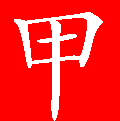
\includegraphics[width=3mm]{../Images/00002}\includegraphics[width=3mm]{../Images/00011}\footnotesize \kaishu 又是不合式{[}之{]}言,擢心语。}抬起脚来咕咚咕咚又跑了。{\includegraphics[width=3mm]{../Images/00002}\includegraphics[width=3mm]{../Images/00011}\footnotesize \kaishu 活龙活现之文。 \includegraphics[width=3mm]{../Images/00004}\includegraphics[width=3mm]{../Images/00011}\footnotesize \kaishu 如画。}红玉便赌气把那样子掷在一边,{\includegraphics[width=3mm]{../Images/00004}\includegraphics[width=3mm]{../Images/00011}\footnotesize \kaishu 何如?}向抽屉内找笔,找了半天都是秃了的,因说道:``前儿一枝新笔,{\includegraphics[width=3mm]{../Images/00004}\includegraphics[width=3mm]{../Images/00011}\footnotesize \kaishu 是补文否?}放在那里了?怎么一时想不起来。''{\includegraphics[width=3mm]{../Images/00004}\includegraphics[width=3mm]{../Images/00011}\footnotesize \kaishu 既在矮檐下,怎敢不低头?}一面说,一面出神,{\includegraphics[width=3mm]{../Images/00002}\includegraphics[width=3mm]{../Images/00011}\footnotesize \kaishu 总是画境。}想了一会方笑道:``是了,前儿晚上莺儿拿了去了。''{\includegraphics[width=3mm]{../Images/00004}\includegraphics[width=3mm]{../Images/00011}\footnotesize \kaishu 还是补文。}便向佳蕙道:``你替我取了来。''佳蕙道:``花大姐姐还等着我替他抬箱子呢,你自取去罢。''红玉道:``他等着你,你还坐着闲打牙儿?{\includegraphics[width=3mm]{../Images/00004}\includegraphics[width=3mm]{../Images/00011}\footnotesize \kaishu 袭人身份。}我不叫你取去,他也不等着你了。坏透了的小蹄子!''说着,自己便出房来,出了怡红院,一径往宝钗院内来。{\includegraphics[width=3mm]{../Images/00004}\includegraphics[width=3mm]{../Images/00011}\footnotesize \kaishu 曲折再四,方逼出正文来。}

刚至沁芳亭畔,只见宝玉的奶娘李嬷嬷从那边走来。{\includegraphics[width=3mm]{../Images/00002}\includegraphics[width=3mm]{../Images/00011}\footnotesize \kaishu 奇文,真令人不得机关。}红玉立住问道:``李奶奶,你老人家那去了?怎打这里来?''李嬷嬷站住,将手一拍道:``你说说,好好的又看上了那个种树的什么云哥儿雨哥儿的,{\includegraphics[width=3mm]{../Images/00002}\includegraphics[width=3mm]{../Images/00011}\footnotesize \kaishu 囫囵不解语。◇奇文神文。}这会子逼着我叫了他来。明儿叫上房里听见,可又是不好。''{\includegraphics[width=3mm]{../Images/00002}\includegraphics[width=3mm]{../Images/00011}\footnotesize \kaishu 更不解。}红玉笑道:``你老人家当真的就依了他去叫了?''{\includegraphics[width=3mm]{../Images/00002}\includegraphics[width=3mm]{../Images/00011}\footnotesize \kaishu 是遂心语。}李嬷嬷道:``可怎么样呢?''{\includegraphics[width=3mm]{../Images/00002}\includegraphics[width=3mm]{../Images/00011}\footnotesize \kaishu 妙!的是老妪口气。}红玉笑道:``那一个要是知道好歹,{\includegraphics[width=3mm]{../Images/00002}\includegraphics[width=3mm]{../Images/00011}\footnotesize \kaishu 更不解。}就回不进来才是。''{\includegraphics[width=3mm]{../Images/00002}\includegraphics[width=3mm]{../Images/00012}\footnotesize \kaishu 是私心语,神妙!}李嬷嬷道:``他又不痴,为什么不进来?''红玉道:``既是来了,你老人家该同他一齐来,回来叫他一个人乱碰,可是不好呢。''{\includegraphics[width=3mm]{../Images/00002}\includegraphics[width=3mm]{../Images/00012}\footnotesize \kaishu 总是私心语,要直问又不敢,只用这等语慢慢套出。有神理。}李嬷嬷道:``我有那样工夫和他走?不过告诉了他,回来打发个小丫头子或是老婆子,带进他来就完了。''说着,拄着拐一径去了。红玉听说,便站着出神,且不去取笔。{\includegraphics[width=3mm]{../Images/00002}\includegraphics[width=3mm]{../Images/00012}\footnotesize \kaishu 总是不言神情,另出花样。}

一时,只见一个小丫头子跑来,见红玉站在那里,便问道:``林姐姐,你在这里作什么呢?''红玉抬头见是小丫头子坠儿。{\includegraphics[width=3mm]{../Images/00002}\includegraphics[width=3mm]{../Images/00012}\footnotesize \kaishu 坠儿者,赘儿也。人生天地间已是赘疣,况又生许多冤情孽债。叹叹!}红玉道:``那去?''坠儿道:``叫我带进芸二爷来。''{\includegraphics[width=3mm]{../Images/00004}\includegraphics[width=3mm]{../Images/00011}\footnotesize \kaishu 等的是这句话。}说着一径跑了。这里红玉刚走至蜂腰桥门前,只见那边坠儿引着贾芸来了。{\includegraphics[width=3mm]{../Images/00002}\includegraphics[width=3mm]{../Images/00012}\footnotesize \kaishu 妙!不说红玉不走,亦不说走,只说``刚走到''三字,可知红玉有私心矣。若说出必定不走必定走,则文字死板,亦且亦棱角过露,非写女儿之笔也。}那贾芸一面走,一面拿眼把红玉一溜;那红玉只装作和坠儿说话,也把眼去一溜贾芸。四目恰相对时,红玉不觉脸红了,{{\includegraphics[width=3mm]{../Images/00002}\includegraphics[width=3mm]{../Images/00012}\footnotesize \kaishu 看官至此,须掩卷细想,上三十回中篇篇句句点``红''字处,可与此处{(想)}{[}相比{]}如何?}}一扭身往蘅芜苑去了。不在话下。

这里贾芸随着坠儿,逶迤来至怡红院中。坠儿先进去回明了,然后方领贾芸进去。贾芸看时,只见院内略略的有几点山石,种着芭蕉,那边有两只仙鹤在松树下剔翎。一溜回廊上吊着各色笼子,各色仙禽异鸟。上面小小五间抱厦,一色雕镂新鲜花样隔扇,上面悬着一个匾额,四个大字题道是``怡红快绿''。贾芸想道:``怪道叫`怡红院',可知原来匾上是恁样四个字。''{\includegraphics[width=3mm]{../Images/00002}\includegraphics[width=3mm]{../Images/00012}\footnotesize \kaishu 伤哉,展眼便红稀绿瘦矣。叹叹!}正想着,只听里面隔着纱窗子笑道:{\includegraphics[width=3mm]{../Images/00002}\includegraphics[width=3mm]{../Images/00011}\footnotesize \kaishu 是文若张僧繇点睛之龙,破壁飞矣,焉得不拍案叫绝!}``快进来罢。我怎么就忘了你两三个月!''贾芸听得是宝玉的声音,连忙进入房内。抬头一看,只见金碧辉煌,{\includegraphics[width=3mm]{../Images/00002}\includegraphics[width=3mm]{../Images/00011}\footnotesize \kaishu 器皿叠叠。 \includegraphics[width=3mm]{../Images/00004}\includegraphics[width=3mm]{../Images/00011}\footnotesize \kaishu 不能细览之文。}文章熌灼,{\includegraphics[width=3mm]{../Images/00002}\includegraphics[width=3mm]{../Images/00011}\footnotesize \kaishu 陈设垒垒。 \includegraphics[width=3mm]{../Images/00004}\includegraphics[width=3mm]{../Images/00011}\footnotesize \kaishu 不得细玩之文。}却看不见宝玉在那里。{\includegraphics[width=3mm]{../Images/00002}\includegraphics[width=3mm]{../Images/00011}\footnotesize \kaishu 武夷九曲之文。}一回头,只见左边立着一架大穿衣镜,从镜后转出两个一般大的十五六岁的丫头来说:``请二爷里头屋里坐。''贾芸连正眼也不敢看,连忙答应了。又进一道碧纱厨,只见一张小小填漆床上,悬着大红销金撒花帐子。宝玉穿着家常衣服,靸着鞋,倚在床上拿着本书看,{\includegraphics[width=3mm]{../Images/00002}\includegraphics[width=3mm]{../Images/00011}\footnotesize \kaishu 这是等芸哥看,故作款式。若果真看书,在隔纱窗子说话时已放下了。玉兄若见此批,必云:老货,他处处不放松我,可恨可恨!回思将余比作钗、颦等,乃一知己,余何幸也!一笑。}见他进来,将书掷下,早堆着笑立起身来。{\includegraphics[width=3mm]{../Images/00004}\includegraphics[width=3mm]{../Images/00011}\footnotesize \kaishu 小叔身段。}贾芸忙上前请了安。宝玉让坐,便在下面一张椅子上坐了。宝玉笑道:``只从那日见了你,我叫你往书房里来,谁知接接连连许多事情,就把你忘了。''贾芸笑道:``总是我没福,偏偏又遇着叔叔身上欠安。叔叔如今可大安了?''宝玉道:``大好了。我倒听见说你辛苦了好几天。''贾芸道:``辛苦也是该当的。叔叔大安了,也是我们一家子的造化。''{\includegraphics[width=3mm]{../Images/00002}\includegraphics[width=3mm]{../Images/00011}\footnotesize \kaishu 不伦不理,迎合字样,口气逼肖,可笑可叹! \includegraphics[width=3mm]{../Images/00004}\includegraphics[width=3mm]{../Images/00011}\footnotesize \kaishu 谁一家子?可发一大笑。}

说着,只见有个丫鬟端了茶来与他。那贾芸口里和宝玉说着话,眼睛却溜瞅那丫鬟:{\includegraphics[width=3mm]{../Images/00002}\includegraphics[width=3mm]{../Images/00011}\footnotesize \kaishu 前写不敢正眼,今又如此写,是因茶来,有心人故留此神,于接茶时站起,方不突然。 \includegraphics[width=3mm]{../Images/00004}\includegraphics[width=3mm]{../Images/00011}\footnotesize \kaishu 此句是认人,非前溜红玉之文。}细挑身材,容长脸面,穿着银红袄子,青缎背心,白绫细折裙。------不是别人,却是袭人。{\includegraphics[width=3mm]{../Images/00002}\includegraphics[width=3mm]{../Images/00011}\footnotesize \kaishu 《水浒》文法用的恰当,是芸哥眼中也。}那贾芸自从宝玉病了,他在里头混了两天,他却把那有名人口认记了一半。{\includegraphics[width=3mm]{../Images/00002}\includegraphics[width=3mm]{../Images/00011}\footnotesize \kaishu 一路总是贾芸是个有心人,一丝不乱。}他也知道袭人在宝玉房中比别个不同,{\includegraphics[width=3mm]{../Images/00004}\includegraphics[width=3mm]{../Images/00011}\footnotesize \kaishu 何如?可知余前批不谬。}今见他端了茶来,宝玉又在旁边坐着,便忙站起来笑道:``姐姐怎么替我倒起茶来。我来到叔叔这里,又不是客,让我自己倒罢了。''{\includegraphics[width=3mm]{../Images/00002}\includegraphics[width=3mm]{../Images/00012}\footnotesize \kaishu 总写贾芸乖觉,一丝不乱。}宝玉道:``你只管坐着罢。丫头们跟前也是这样。''贾芸笑道:``虽如此说,叔叔房里姐姐们,我怎么敢放肆呢?''{\includegraphics[width=3mm]{../Images/00002}\includegraphics[width=3mm]{../Images/00011}\footnotesize \kaishu 红玉何以使得?}一面说,一面坐下吃茶。

那宝玉便和他说些没要紧的散话。{{\includegraphics[width=3mm]{../Images/00002}\includegraphics[width=3mm]{../Images/00012}\footnotesize \kaishu 妙极是极!况宝玉又有何正{(紧)}{[}经{]}可说的! \includegraphics[width=3mm]{../Images/00004}\includegraphics[width=3mm]{../Images/00012}\footnotesize \kaishu 此批被作者偏过了。}}又说道谁家的戏子好,谁家的花园好,又告诉他谁家的丫头标致,谁家的酒席丰盛,又是谁家有奇货,又是谁家有异物。{{\includegraphics[width=3mm]{../Images/00002}\includegraphics[width=3mm]{../Images/00012}\footnotesize \kaishu 几个``谁家'',自北静王、公侯驸马诸大家包括尽矣,写尽纨绔口角。 }\includegraphics[width=3mm]{../Images/00004}\includegraphics[width=3mm]{../Images/00012}\footnotesize \kaishu 脂砚斋再笔:对芸兄原无可说之话。}那贾芸口里只得顺着他说,说了一回,见宝玉有些懒懒的了,便起身告辞。宝玉也不甚留,只说:``你明儿闲了,只管来。''仍命小丫头子坠儿送他出去。

出了怡红院,贾芸见四顾无人,便把脚慢慢的停着些走,口里一长一短和坠儿说话,先问他``几岁了?名字叫什么?你父母在那一行上?在宝叔房内几年了?{\includegraphics[width=3mm]{../Images/00002}\includegraphics[width=3mm]{../Images/00011}\footnotesize \kaishu 渐渐入港。}一个月多少钱?共总宝叔房内有几个女孩子?''那坠儿见问,便一桩桩的都告诉他了。贾芸又道:``刚才那个与你说话的,他可是叫小红?''坠儿笑道:``他倒叫小红。你问他作什么?''贾芸道:``方才他问你什么手帕子,我倒拣了一块。''坠儿听了笑道:``他问了我好几遍,可有看见他的帕子。我有那么大工夫管这些事!今儿他又问我,他说我替他找着了,他还谢我呢。{\includegraphics[width=3mm]{../Images/00004}\includegraphics[width=3mm]{../Images/00011}\footnotesize \kaishu ``传''字正文,此处方露。}才在蘅芜苑门口说的,二爷也听见了,不是我撒谎。好二爷,你既拣着了,给我罢。我看他拿什么谢我。''

原来上月贾芸进来种树之时,便拣了一块罗帕,便知是所在园内的人失落的,但不知是那一个人的,故不敢造次。今儿听见红玉问坠儿,便知是红玉的,心内不胜喜幸。又见坠儿追索,心中早得了主意,便向袖内将自己的一块取了出来,向坠儿笑道:``我给是给你,你若得了他的谢礼,可不许瞒着我。''坠儿满口里答应了,接了手帕子,送出贾芸,回来找红玉,不在话下。{\includegraphics[width=3mm]{../Images/00002}\includegraphics[width=3mm]{../Images/00012}\footnotesize \kaishu 至此一顿,狡猾之甚!原非书中正文之人,写来间色耳。}

如今且说宝玉打发了贾芸去后,意思懒懒的歪在床上,似有朦胧之态。袭人便走上来,坐在床沿上推他,说道:``怎么又要睡觉?闷的很,你出去逛逛不是?''宝玉见说,便拉他的手笑道:``我要去,只是舍不得你。''袭人笑道:``快起来罢!''{\includegraphics[width=3mm]{../Images/00002}\includegraphics[width=3mm]{../Images/00011}\footnotesize \kaishu 不答得妙! \includegraphics[width=3mm]{../Images/00004}\includegraphics[width=3mm]{../Images/00011}\footnotesize \kaishu 不答上文,妙极!}一面说,一面拉了宝玉起来。宝玉道:``可往那里去呢?怪腻腻烦烦的。''{\includegraphics[width=3mm]{../Images/00004}\includegraphics[width=3mm]{../Images/00011}\footnotesize \kaishu 玉兄最得意之文,起笔却如此写。}袭人道:``你出去了就好了。只管这么葳蕤,越发心里烦腻。''

宝玉无精打采的,只得依他。晃出了房门,在回廊上调弄了一回雀儿;出至院外,顺着沁芳溪看了一回金鱼。只见那边山坡上两只小鹿箭也似的跑来,宝玉不解何意,{\includegraphics[width=3mm]{../Images/00002}\includegraphics[width=3mm]{../Images/00011}\footnotesize \kaishu 余亦不解。}正自纳闷,只见贾兰在后面拿着一张小弓追了下来。{\includegraphics[width=3mm]{../Images/00002}\includegraphics[width=3mm]{../Images/00011}\footnotesize \kaishu 前文。 \includegraphics[width=3mm]{../Images/00004}\includegraphics[width=3mm]{../Images/00011}\footnotesize \kaishu 此等文可是人能意料的?}一见宝玉在前面,便站住了,笑道:``二叔叔在家里呢,我只当出门去了。''宝玉道:``你又淘气了。好好的射他作什么?''贾兰笑道:``这会子不念书,闲着作什么?所以演习演习骑射。''{\includegraphics[width=3mm]{../Images/00002}\includegraphics[width=3mm]{../Images/00011}\footnotesize \kaishu 奇文奇语,默思之方意会。为玉兄之毫无一正事,只知安富尊荣而写。 \includegraphics[width=3mm]{../Images/00004}\includegraphics[width=3mm]{../Images/00011}\footnotesize \kaishu 答的何其堂皇正大,何其坦然之至!}宝玉道:``把牙栽了,那时才不演呢。''

说着,顺着脚一径来至一个院门前,{\includegraphics[width=3mm]{../Images/00004}\includegraphics[width=3mm]{../Images/00011}\footnotesize \kaishu 像无意。}只见凤尾森森,龙吟细细。{\includegraphics[width=3mm]{../Images/00002}\includegraphics[width=3mm]{../Images/00012}\footnotesize \kaishu 与后文``落叶萧萧,寒烟漠漠''一对,可伤可叹!}举目望门上一看,{\includegraphics[width=3mm]{../Images/00002}\includegraphics[width=3mm]{../Images/00011}\footnotesize \kaishu 无一丝心机,反似初至者,故接有忘形忘情话来。 \includegraphics[width=3mm]{../Images/00004}\includegraphics[width=3mm]{../Images/00011}\footnotesize \kaishu 原无意。}只见匾上写着``潇湘馆''三字。{\includegraphics[width=3mm]{../Images/00004}\includegraphics[width=3mm]{../Images/00011}\footnotesize \kaishu 三字如此出,足见真出无意。}宝玉信步走入,只见湘帘垂地,悄无人声。走至窗前,觉得一缕幽香从碧纱窗中暗暗透出。{\includegraphics[width=3mm]{../Images/00002}\includegraphics[width=3mm]{../Images/00011}\footnotesize \kaishu 写得出,写得出。}宝玉便将脸贴在纱窗上,往里看时,耳内忽听得{\includegraphics[width=3mm]{../Images/00002}\includegraphics[width=3mm]{../Images/00012}\footnotesize \kaishu 未曾看见先听见,有神理。}细细的长叹了一声道:``\,`每日家情思睡昏昏'。''{\includegraphics[width=3mm]{../Images/00002}\includegraphics[width=3mm]{../Images/00011}\footnotesize \kaishu 用情忘情,神化之文。 \includegraphics[width=3mm]{../Images/00004}\includegraphics[width=3mm]{../Images/00010}\footnotesize \kaishu 先用``凤尾森森,龙吟细细''八字,``一缕幽香自纱窗中暗暗透出'',``细细的长叹一声''等句,方引出``每日家情思睡昏昏''仙音妙音来,非纯化功夫之笔不能,可见行文之难。}宝玉听了,不觉心内痒将起来,再看时,只见黛玉在床上伸懒腰。{\includegraphics[width=3mm]{../Images/00002}\includegraphics[width=3mm]{../Images/00011}\footnotesize \kaishu 有神理,真真画出。}宝玉在窗外笑道:``为甚么`每日家情思睡昏昏'?''一面说,一面掀帘进来了。{\includegraphics[width=3mm]{../Images/00004}\includegraphics[width=3mm]{../Images/00010}\footnotesize \kaishu 二玉这回文字,作者亦在无意上写来,所谓``信手拈来无不是''也。}

林黛玉自觉忘情,不觉红了脸,拿袖子遮了脸,翻身向里装睡着了。宝玉才走上来要搬他的身子,只见黛玉的奶娘并两个婆子却跟了进来{\includegraphics[width=3mm]{../Images/00002}\includegraphics[width=3mm]{../Images/00011}\footnotesize \kaishu 一丝不漏,且避若干嚼蜡之文。}说:``妹妹睡觉呢,等醒了再请来。''刚说着,黛玉便翻身向外坐起来,笑道:``谁睡觉呢?''{\includegraphics[width=3mm]{../Images/00002}\includegraphics[width=3mm]{../Images/00011}\footnotesize \kaishu 妙极!可知黛玉是怕宝玉去也。}那两三个婆子见黛玉起来,便笑道:``我们只当姑娘睡着了。''说着,便叫紫鹃说:``姑娘醒了,进来伺候。''一面说,一面都去了。

黛玉坐在床上,一面抬手整理鬓发,一面笑向宝玉道:``人家睡觉,你进来作什么?''宝玉见他星眼微饧,香腮带赤,不觉神魂早荡,一歪身坐在椅子上,笑道:``你才说什么?''黛玉道:``我没说什么。''宝玉笑道:``给你个榧子呢,我都听见了。''

二人正说话,只见紫鹃进来。宝玉笑道:``紫鹃,把你们的好茶倒碗我吃。''紫鹃道:``那里是好的呢?要好的,只是等袭人来。''黛玉道:``别理他,你先给我舀水去罢。''紫鹃笑道:``他是客,自然先倒了茶来再舀水去。''说着倒茶去了。宝玉笑道:``好丫头,`若共你多情小姐同鸳帐,怎舍得叠被铺床?'''{\includegraphics[width=3mm]{../Images/00002}\includegraphics[width=3mm]{../Images/00011}\footnotesize \kaishu 真正无意忘情。 \includegraphics[width=3mm]{../Images/00004}\includegraphics[width=3mm]{../Images/00011}\footnotesize \kaishu 真正无意忘情冲口而出之语。 \includegraphics[width=3mm]{../Images/00004}\includegraphics[width=3mm]{../Images/00010}\footnotesize \kaishu 方才见芸哥所拿之书一定是《西厢》,不然如何忘情至此?}林黛玉登时撂下脸来,{\includegraphics[width=3mm]{../Images/00002}\includegraphics[width=3mm]{../Images/00011}\footnotesize \kaishu 我也要恼。}说道:``二哥哥,你说什么?''宝玉笑道:``我何尝说什么。''黛玉便哭道:``如今新兴的,外头听了村话来,也说给我听;看了混帐书,也来拿我取笑儿。我成了替爷们解闷的。''一面哭着,一面下床来,往外就走。宝玉不知要怎样,心下慌了,忙赶上来,``好妹妹,我一时该死,你别告诉去。我再要敢,嘴上就长个疔,烂了舌头。''

正说着,只见袭人走来说道:``快回去穿衣服,老爷叫你呢。''{\includegraphics[width=3mm]{../Images/00004}\includegraphics[width=3mm]{../Images/00010}\footnotesize \kaishu 若无如此文字收拾二玉,写颦无非至再哭恸哭,玉只以赔尽小心软求慢恳,二人一笑而止。且书内若此亦多多矣,未免有犯雷同之病。故用险句结住,使二玉心中不得不将现事抛却,各怀一惊心意,再作下文。壬午孟夏,雨窗。畸笏。}宝玉听了,不觉的打了个焦雷的一般,{\includegraphics[width=3mm]{../Images/00002}\includegraphics[width=3mm]{../Images/00011}\footnotesize \kaishu 不止玉兄一惊,即阿颦亦不免一吓,作者只顾写来收拾二玉之文,忘却颦儿也。想作者亦似宝玉道《西厢》之句,忘情而出也。{[}呵呵{]}}也顾不得别的,急忙回来穿衣服。出园来,只见茗烟在二门前等着,宝玉便问道:``是作什么?''茗烟道:``爷快出来罢,横竖是见去的,到那里就知道了。''一面说,一面催着宝玉。

转过大厅,宝玉心里还自狐疑,只听墙角边一阵呵呵大笑,回头看时,见是薛蟠拍着手跳了出来,笑道:{\includegraphics[width=3mm]{../Images/00002}\includegraphics[width=3mm]{../Images/00011}\footnotesize \kaishu 如此戏弄,非呆兄无人。欲释二玉,非此戏弄不能立解,勿得泛泛看过。不知作者胸中有多少丘壑。 \includegraphics[width=3mm]{../Images/00004}\includegraphics[width=3mm]{../Images/00011}\footnotesize \kaishu 非呆兄行不出此等戏弄,但作者有多少丘壑在胸中,写来酷肖。}``要不说姨夫叫你,你那里出来的这么快。''茗烟也笑着跪下了。宝玉怔了半天,方解过来是薛蟠哄他出来。薛蟠连忙打恭作揖陪不是,{\includegraphics[width=3mm]{../Images/00004}\includegraphics[width=3mm]{../Images/00011}\footnotesize \kaishu 酷肖。}又求``不要难为了小子,都是我逼他去的''。宝玉也无法了,只好笑,因说道:``你哄我也罢了,怎么说我父亲呢?我告诉姨娘去,评评这个理,可使得么?''薛蟠忙道:``好兄弟,我原为求你快些出来,就忘了忌讳这句话。改日你也哄我,说我的父亲就完了。''{\includegraphics[width=3mm]{../Images/00002}\includegraphics[width=3mm]{../Images/00011}\footnotesize \kaishu 写粗豪无心人毕肖。 \includegraphics[width=3mm]{../Images/00004}\includegraphics[width=3mm]{../Images/00011}\footnotesize \kaishu 真真乱话。}宝玉道:``嗳,嗳,越发该死了!''又向茗烟道:``反叛肏的,还跪着作什么!''茗烟连忙叩头起来。薛蟠道:``要不是我也不敢惊动,只因明儿五月初三日是我的生日,谁知古董行的程日兴,他不知那里寻了来的这么粗、这么长粉脆的鲜藕,{\includegraphics[width=3mm]{../Images/00004}\includegraphics[width=3mm]{../Images/00011}\footnotesize \kaishu 如见如闻。}这么大的大西瓜,这么长的一尾新鲜的鲟鱼,这么大的一个暹罗国进贡的灵柏香熏的暹猪。你说,他这四样礼可难得不难得?那鱼、猪不过贵而难得,这藕和瓜亏他怎么种出来的。我连忙孝敬了母亲,赶着给你们老太太、姨父、姨母送了些去。如今留了些,我要自己吃,恐怕折福,{\includegraphics[width=3mm]{../Images/00002}\includegraphics[width=3mm]{../Images/00011}\footnotesize \kaishu 呆兄亦有此语,批书人至此诵《往生咒》至恒河沙数也。}左思右想,除我之外,惟有你还配吃,{\includegraphics[width=3mm]{../Images/00002}\includegraphics[width=3mm]{../Images/00011}\footnotesize \kaishu 此语令人哭不得笑不得,亦真心语也。}所以特请你来。可巧唱曲儿的一个小子又才来了,我同你乐一日何如?''

一面说,一面来至他书房里。只见詹光、程日兴、胡斯来、单聘仁等并唱曲儿的都在这里,见他进来,请安的,问好的,都彼此见过了。吃了茶,薛蟠即命人摆酒来。说犹未了,众小厮七手八脚摆了半天,{\includegraphics[width=3mm]{../Images/00004}\includegraphics[width=3mm]{../Images/00011}\footnotesize \kaishu 又一个写法。}才停当归坐。宝玉果见瓜藕新异,因笑道:``我的寿礼还未送来,倒先扰了。''薛蟠道:``可是呢,明儿你送我什么?''{\includegraphics[width=3mm]{../Images/00004}\includegraphics[width=3mm]{../Images/00011}\footnotesize \kaishu 逼真,酷肖。}宝玉道:``我可有什么可送的?若论银钱吃穿等类的东西,{\includegraphics[width=3mm]{../Images/00002}\includegraphics[width=3mm]{../Images/00011}\footnotesize \kaishu 谁说得出?经过者方说得出。叹叹!}究竟还不是我的,惟有或写一张字,画一张画,才算是我的。''

薛蟠笑道:``你提画儿,我才想起来了。昨儿我看人家一张春宫,{\includegraphics[width=3mm]{../Images/00004}\includegraphics[width=3mm]{../Images/00011}\footnotesize \kaishu 阿呆兄所见之画也!}画的着实好。上面还有许多的字,我也没细看,只看落的款,是`庚黄'{\includegraphics[width=3mm]{../Images/00002}\includegraphics[width=3mm]{../Images/00011}\footnotesize \kaishu 奇文,奇文!}画的。真真好的了不得!''宝玉听说,心下猜疑道:``古今字画也都见过些,那里有个`庚黄'?''想了半天,不觉笑将起来,命人取过笔来,在手心里写了两个字,又问薛蟠道:``你看真了是`庚黄'?''薛蟠道:``怎么看不真!''{\includegraphics[width=3mm]{../Images/00002}\includegraphics[width=3mm]{../Images/00010}\footnotesize \kaishu 闲事顺笔,骂死不学之纨绔。叹叹!{[}壬午雨窗。畸笏。{]}}宝玉将手一撒,与他看道:``别是这两个字罢?其实与`庚黄'相去不远。''众人都看时,原来是``唐寅''两个字,都笑道:``想必是这两字,大爷一时眼花了也未可知。''薛蟠自觉没意思,{\includegraphics[width=3mm]{../Images/00004}\includegraphics[width=3mm]{../Images/00011}\footnotesize \kaishu 实心人。}笑道:``谁知他`糖银'`果银'的。''

正说着,小厮来回:``冯大爷来了。''宝玉便知是神武将军冯唐之子冯紫英来了。薛蟠等一齐都叫:``快请。''说犹未了,只见冯紫英一路说笑{\includegraphics[width=3mm]{../Images/00004}\includegraphics[width=3mm]{../Images/00011}\footnotesize \kaishu 如见如闻。}已进来。{\includegraphics[width=3mm]{../Images/00002}\includegraphics[width=3mm]{../Images/00011}\footnotesize \kaishu 一派英气如在纸上,特为金闺润色也。}众人忙起席让坐。冯紫英笑道:``好呀!也不出门了,在家里高乐罢。''
{\includegraphics[width=3mm]{../Images/00004}\includegraphics[width=3mm]{../Images/00011}\footnotesize \kaishu 如见其人于纸上。}宝玉、薛蟠都笑道:``一向少会,老世伯身上康健?''紫英答道:``家父倒也托庇康健。近来家母偶着了些风寒,不好了两天。''{{\includegraphics[width=3mm]{../Images/00004}\includegraphics[width=3mm]{../Images/00010}\footnotesize \kaishu 紫英豪侠小小一段,是为金闺间色之文,壬午雨窗。}◇写倪二、紫英、湘莲、玉菡侠文,皆各得传真写照之笔。丁亥夏。畸笏叟。◇惜``卫若兰射圃''文字迷失无稿。叹叹!丁亥夏。畸笏叟。}薛蟠见他面上有些青伤,便笑道:``这脸上又和谁挥拳的?挂了幌子了。''冯紫英笑道:``从那一遭把仇都尉的儿子打伤了,我就记了再不怄气,如何又挥拳?这个脸上,是前日打围,在铁网山教兔鹘捎一翅膀。''{\includegraphics[width=3mm]{../Images/00004}\includegraphics[width=3mm]{../Images/00011}\footnotesize \kaishu 如何着想?新奇字样。}宝玉道:``几时的话?''紫英道:``三月二十八日去的,前儿也就回来了。''宝玉道:``怪道前儿初三四儿,我在沈世兄家赴席不见你呢。我要问,不知怎么就忘了。单你去了,还是老世伯也去了?''紫英道:``可不是家父去,我没法儿,去罢了。难道我闲疯了,咱们几个人吃酒听唱不乐,寻那个苦恼去?这一次,大不幸之中又大幸。''{\includegraphics[width=3mm]{../Images/00002}\includegraphics[width=3mm]{../Images/00011}\footnotesize \kaishu 似又伏一大事样,英侠人累累如是,令人猜摹。}

薛蟠众人见他吃完了茶,都说道:``且入席,有话慢慢的说。''{\includegraphics[width=3mm]{../Images/00004}\includegraphics[width=3mm]{../Images/00011}\footnotesize \kaishu 馀文再述。}冯紫英听说,便立起身来说道:``论礼,我该陪饮几杯才是,只是今儿有一件大大要紧事,回去还要见家父面回,实不敢领。''薛蟠、宝玉众人那里肯依,死拉着不放。冯紫英笑道:``这又奇了。{\includegraphics[width=3mm]{../Images/00004}\includegraphics[width=3mm]{../Images/00011}\footnotesize \kaishu 如闻如见。}你我这些年,那一回有这个道理的?果然不能遵命。若必定叫我领,拿大杯来,{\includegraphics[width=3mm]{../Images/00004}\includegraphics[width=3mm]{../Images/00011}\footnotesize \kaishu 写豪爽人如此。}我领两杯就是了。''众人听说,只得罢了,薛蟠执壶,宝玉把盏,斟了两大海。那冯紫英站着,一气而尽。{\includegraphics[width=3mm]{../Images/00002}\includegraphics[width=3mm]{../Images/00011}\footnotesize \kaishu 令人快活煞。 \includegraphics[width=3mm]{../Images/00004}\includegraphics[width=3mm]{../Images/00011}\footnotesize \kaishu 爽快人如此,令人羡煞。}宝玉道:``你到底把这个`不幸之幸'说完了再走。''冯紫英笑道:``今儿说的也不尽兴。我为这个,还要特治一东,请你们去细谈一谈;二则还有所恳之处。''说着执手就走。薛蟠道:``越发说的人热剌剌的丢不下。多早晚才请我们,告诉了也免的人犹豫。''{\includegraphics[width=3mm]{../Images/00004}\includegraphics[width=3mm]{../Images/00011}\footnotesize \kaishu 实心人如此,丝毫形迹俱无,令人痛快煞。}冯紫英道:``多者十日,少则八天。''一面说,一面出门上马去了。众人回来,依席又饮了一回方散。{\includegraphics[width=3mm]{../Images/00002}\includegraphics[width=3mm]{../Images/00011}\footnotesize \kaishu 收拾得好。}

宝玉回至园中,袭人正记挂着他去见贾政,{\includegraphics[width=3mm]{../Images/00002}\includegraphics[width=3mm]{../Images/00011}\footnotesize \kaishu ``生员切己之事'',时刻难忘。}不知是祸是福,{\includegraphics[width=3mm]{../Images/00004}\includegraphics[width=3mm]{../Images/00011}\footnotesize \kaishu 下文伏线。}只见宝玉醉醺醺的回来,问其原故,宝玉一一向他说了。袭人道:``人家牵肠挂肚的等着,你且高乐去,也到底打发人来给个信儿。''宝玉道:``我何尝不要送信儿,只因冯世兄来了,就混忘了。''

正说着,只见宝钗走进来笑道:``偏了我们新鲜东西了。''宝玉笑道:``姐姐家的东西,自然先偏了我们了。''宝钗摇头笑道:``昨儿哥哥倒特特的请我吃,我不吃他,叫他留着送人请人罢。我知道我的命小福薄,不配吃那个。''{\includegraphics[width=3mm]{../Images/00002}\includegraphics[width=3mm]{../Images/00011}\footnotesize \kaishu 暗对呆兄言宝玉配吃语。}说着,丫鬟倒了茶来,吃茶说闲话儿,不在话下。

却说那林黛玉听见贾政叫了宝玉去了,一日不回来,心中也替他忧虑。{\includegraphics[width=3mm]{../Images/00002}\includegraphics[width=3mm]{../Images/00011}\footnotesize \kaishu 本是切己事。}至晚饭后,闻听宝玉来了,心里要找他问问是怎么样了。{\includegraphics[width=3mm]{../Images/00002}\includegraphics[width=3mm]{../Images/00011}\footnotesize \kaishu 呆兄此席,的是合和筵也。一笑。 \includegraphics[width=3mm]{../Images/00004}\includegraphics[width=3mm]{../Images/00011}\footnotesize \kaishu 这席东道是和事酒不是?}一步步行来,见宝钗进宝玉的院内去了,{\includegraphics[width=3mm]{../Images/00002}\includegraphics[width=3mm]{../Images/00011}\footnotesize \kaishu 《石头记》最好看处是此等章法。}自己也便随后走了来。刚到了沁芳桥,只见各色水禽都在池中浴水,也认不出名色来,但见一个个文彩炫耀,好看异常,因而站住看了一回。{\includegraphics[width=3mm]{../Images/00004}\includegraphics[width=3mm]{../Images/00011}\footnotesize \kaishu 避难法。}再往怡红院来,只见院门关着,黛玉便以手扣门。

谁知晴雯和碧痕正拌了嘴,没好气,忽见宝钗来了,那晴雯正把气移在宝钗身上,{\includegraphics[width=3mm]{../Images/00004}\includegraphics[width=3mm]{../Images/00010}\footnotesize \kaishu 晴雯迁怒是常事耳,写钗、颦二卿身上,与踢袭人之文,令人于何处设想着笔?丁亥夏。畸笏叟。}正在院内抱怨说:``有事没事跑了来坐着,{\includegraphics[width=3mm]{../Images/00002}\includegraphics[width=3mm]{../Images/00011}\footnotesize \kaishu 犯宝钗如此写法。}叫我们三更半夜不得睡觉!''{\includegraphics[width=3mm]{../Images/00002}\includegraphics[width=3mm]{../Images/00011}\footnotesize \kaishu 指明人,则暗写。}忽听又有人叫门,晴雯越发动了气,也并不问是谁,{\includegraphics[width=3mm]{../Images/00002}\includegraphics[width=3mm]{../Images/00011}\footnotesize \kaishu 犯黛玉如此写明。}便说道:``都睡下了,明儿再来罢!''{\includegraphics[width=3mm]{../Images/00002}\includegraphics[width=3mm]{../Images/00011}\footnotesize \kaishu 不知人,则明写。}林黛玉素知丫头们的情性,他们彼此顽耍惯了,恐怕院内的丫头没听真是他的声音,只当是别的丫头们来了,所以不开门,因而又高声说道:``是我,还不开么?''晴雯偏生还没听出来,{\includegraphics[width=3mm]{../Images/00002}\includegraphics[width=3mm]{../Images/00011}\footnotesize \kaishu 想黛玉高声亦不过你我平常说话一样耳,况晴雯素昔浮躁多气之人,如何辨得出?此刻须得批书人唱``大江东去''的喉咙,嚷着``是我林黛玉叫门''方可。又想若开了门,如何有后面很多好字样好文章,看官者意为是否?}便使性子说道:``凭你是谁,二爷吩咐的,一概不许放人进来呢!''林黛玉听了,不觉气怔在门外,待要高声问他,斗起气来,自己又回思一番:``虽说是舅母家如同自己家一样,到底是客边。{\includegraphics[width=3mm]{../Images/00002}\includegraphics[width=3mm]{../Images/00011}\footnotesize \kaishu 寄食者着眼,况颦儿何等人乎?}如今父母双亡,无依无靠,现在他家依栖。如今认真淘气,也觉没趣。''一面想,一面又滚下泪珠来。正是回去不是,站着不是。正没主意,只听里面一阵笑语之声,细听了一听,竟是宝玉、宝钗二人。林黛玉心中益发动了气,左思右想,忽然想起早起的事来:``必定是宝玉恼我告他的原故。但只我何尝告你去了,你也不打听打听,就恼我到这步田地。你今儿不叫我进来,难道明儿就不见面了!''越想越伤感,也不顾苍苔露冷,花径风寒,独立墙角边花阴之下,悲悲戚戚呜咽起来。{\includegraphics[width=3mm]{../Images/00002}\includegraphics[width=3mm]{../Images/00011}\footnotesize \kaishu 可怜杀!可疼杀!余亦泪下。}

原来这林黛玉秉绝代姿容,具希世俊美,不期这一哭,那附近柳枝花朵上的宿鸟栖鸦一闻此声,俱忒楞楞飞起远避,不忍再听。{\includegraphics[width=3mm]{../Images/00002}\includegraphics[width=3mm]{../Images/00011}\footnotesize \kaishu 沉鱼落雁,闭月羞花,原来是哭出来的。一笑。}真是:

花魂默默无情绪,鸟梦痴痴何处惊。

因有一首诗道:

颦儿才貌世应希,独抱幽芳出绣闺;

呜咽一声犹未了,落花满地鸟惊飞。

那林黛玉正自啼哭,忽听``吱喽''一声,院门开处,不知是那一个出来。且看下回。{\includegraphics[width=3mm]{../Images/00002}\includegraphics[width=3mm]{../Images/00012}\footnotesize \kaishu 每阅此本,掩卷者十有八九,不忍下阅看完,想作者此时泪下如豆矣。}

\includegraphics[width=3mm]{../Images/00002}{此回乃颦儿正文,故借小红许多曲折琐碎之笔作引。}

{怡红院见贾芸,宝玉心内似有如无,贾芸眼中应接不暇。}

{``凤尾森森,龙吟细细''八字,``一缕幽香从碧纱窗中暗暗透出'',又``细细的长叹一声''等句方引出``每日家情思睡昏昏''仙音妙音,俱纯化工夫之笔。}

{二玉这回文字,作者亦在无意上写来,所谓``信手拈来无不是''也。}

{收拾二玉文字,写颦无非哭玉、再哭、恸哭,玉只以陪事小心软求慢恳,二人一笑而止。且书内若此亦多多矣,未免有犯雷同之病。故险语结住,使二玉心中不得不将现事抛却,各怀以惊心意,再作下文。}

{前回倪二、紫英、湘莲、玉菡四样侠文皆得传真写照之笔。惜``卫若兰射圃''文字迷失无稿,叹叹!}

{晴雯迁怒系常事耳,写于钗、颦二卿身上,与踢袭人、打平儿之文,令人于何处设想着笔。}

{黛玉望怡红之泣,是``每日家情思睡昏昏''上来。}

{\includegraphics[width=3mm]{../Images/00005}总评:喜相逢,三生注定;遗手帕,月老红丝。幸得人语说连理,又忽见他枝并蒂。难猜未解细追思,罔多疑,空向花枝哭月底。}
